\section{Projekt Bazy Danych}
    \subsection{Model bazy danych - relacyjna SQL}
        Baza danych jest relacyjna oraz obsługiwana jest na serwerze SQL.
    \subsection{Opis}

        \subsubsection{Ustawienie uprawnień dla użytkownika}
        \begin{lstlisting}
CREATE USER 'projekt'@'localhost' IDENTIFIED BY 'Pracownia107!'; 
GRANT ALL PRIVILEGES ON pilkanozna.* TO 'projekt'@'localhost';
        \end{lstlisting}

    \subsection{Rysunek}
        \begin{figure}[!htb]
            \centering
            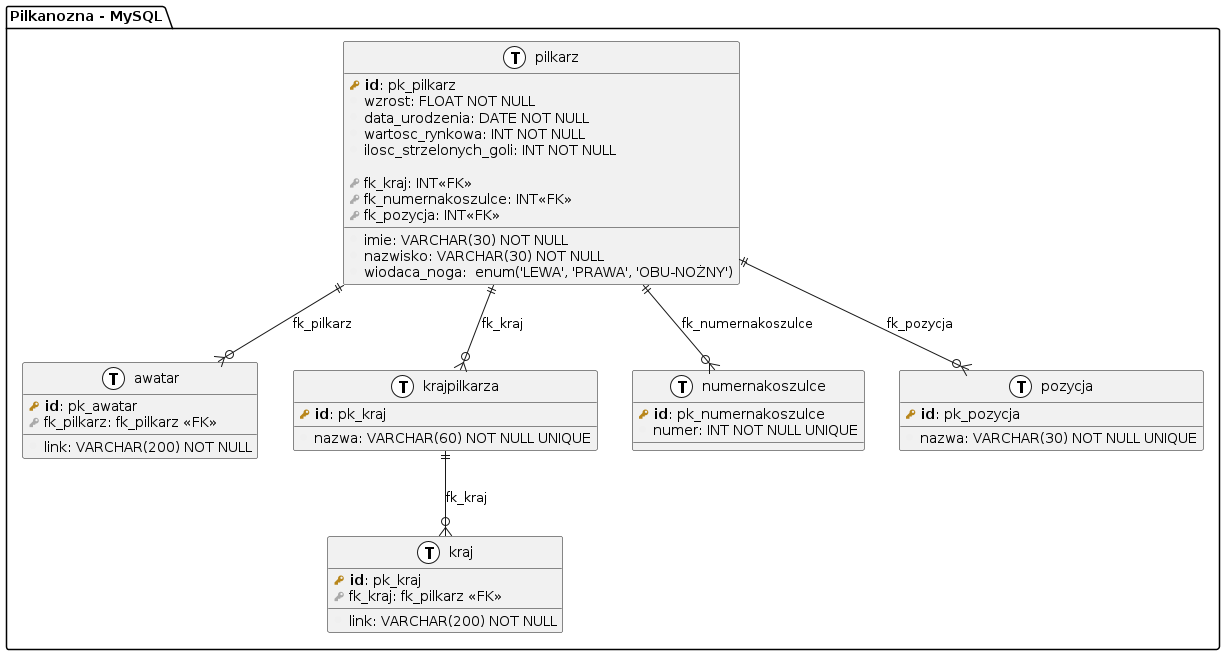
\includegraphics[width=0.9\textwidth]{diagramy/bazy.png}
            \caption{Diagram tabel bazy danych pilkanozna}
        \end{figure}